
\tikzset{every picture/.style={line width=0.75pt}} %set default line width to 0.75pt        

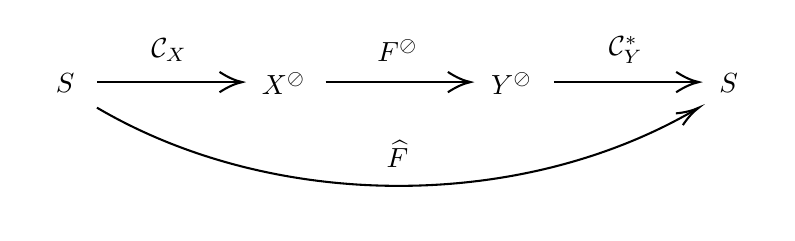
\begin{tikzpicture}[x=0.75pt,y=0.75pt,yscale=-1,xscale=1]
%uncomment if require: \path (0,629); %set diagram left start at 0, and has height of 629

%Straight Lines [id:da560650477859397] 
\draw    (210.17,60.86) -- (278,60.86) ;
\draw [shift={(280,60.86)}, rotate = 180] [color={rgb, 255:red, 0; green, 0; blue, 0 }  ][line width=0.75]    (10.93,-4.9) .. controls (6.95,-2.3) and (3.31,-0.67) .. (0,0) .. controls (3.31,0.67) and (6.95,2.3) .. (10.93,4.9)   ;
%Curve Lines [id:da8170296687430567] 
\draw    (210,73.17) .. controls (295.24,123.25) and (414.47,123.33) .. (498.73,73.92) ;
\draw [shift={(500,73.17)}, rotate = 149.25] [color={rgb, 255:red, 0; green, 0; blue, 0 }  ][line width=0.75]    (10.93,-3.29) .. controls (6.95,-1.4) and (3.31,-0.3) .. (0,0) .. controls (3.31,0.3) and (6.95,1.4) .. (10.93,3.29)   ;
%Straight Lines [id:da24312545548628428] 
\draw    (320.17,60.86) -- (388,60.86) ;
\draw [shift={(390,60.86)}, rotate = 180] [color={rgb, 255:red, 0; green, 0; blue, 0 }  ][line width=0.75]    (10.93,-4.9) .. controls (6.95,-2.3) and (3.31,-0.67) .. (0,0) .. controls (3.31,0.67) and (6.95,2.3) .. (10.93,4.9)   ;
%Straight Lines [id:da8363047188359607] 
\draw    (430.17,60.86) -- (498,60.86) ;
\draw [shift={(500,60.86)}, rotate = 180] [color={rgb, 255:red, 0; green, 0; blue, 0 }  ][line width=0.75]    (10.93,-4.9) .. controls (6.95,-2.3) and (3.31,-0.67) .. (0,0) .. controls (3.31,0.67) and (6.95,2.3) .. (10.93,4.9)   ;

% Text Node
\draw (194.75,61.35) node  [  ] [align=left] {\begin{minipage}[lt]{20.51pt}\setlength\topsep{0pt}
\begin{center}
$S$
\end{center}

\end{minipage}};
% Text Node
\draw (300,61.35) node  [  ] [align=left] {\begin{minipage}[lt]{27.2pt}\setlength\topsep{0pt}
\begin{center}
$X^\oslash$
\end{center}

\end{minipage}};
% Text Node
\draw (409.83,61.35) node  [  ] [align=left] {\begin{minipage}[lt]{26.97pt}\setlength\topsep{0pt}
\begin{center}
$Y^\oslash$
\end{center}

\end{minipage}};
% Text Node
\draw (514.42,61.35) node  [  ] [align=left] {\begin{minipage}[lt]{20.51pt}\setlength\topsep{0pt}
\begin{center}
$S$
\end{center}

\end{minipage}};
% Text Node
\draw (244.83,45.51) node  [  ] [align=left] {\begin{minipage}[lt]{47.83pt}\setlength\topsep{0pt}
\begin{center}
$\mathcal{C}_X$
\end{center}

\end{minipage}};
% Text Node
\draw (354.83,45.51) node  [  ] [align=left] {\begin{minipage}[lt]{47.83pt}\setlength\topsep{0pt}
\begin{center}
$F^\oslash$
\end{center}

\end{minipage}};
% Text Node
\draw (464.83,45.51) node  [  ] [align=left] {\begin{minipage}[lt]{47.83pt}\setlength\topsep{0pt}
\begin{center}
$\mathcal{C}_Y^*$
\end{center}

\end{minipage}};
% Text Node
\draw (354.83,95.51) node  [  ] [align=left] {\begin{minipage}[lt]{47.83pt}\setlength\topsep{0pt}
\begin{center}
$\widehat{F}$
\end{center}

\end{minipage}};


\end{tikzpicture}
